% --------------------------------------------------------------------
% Anexos -------------------------------------------------------------

% Código para agregar el informe académico en formato PDF ------------
% 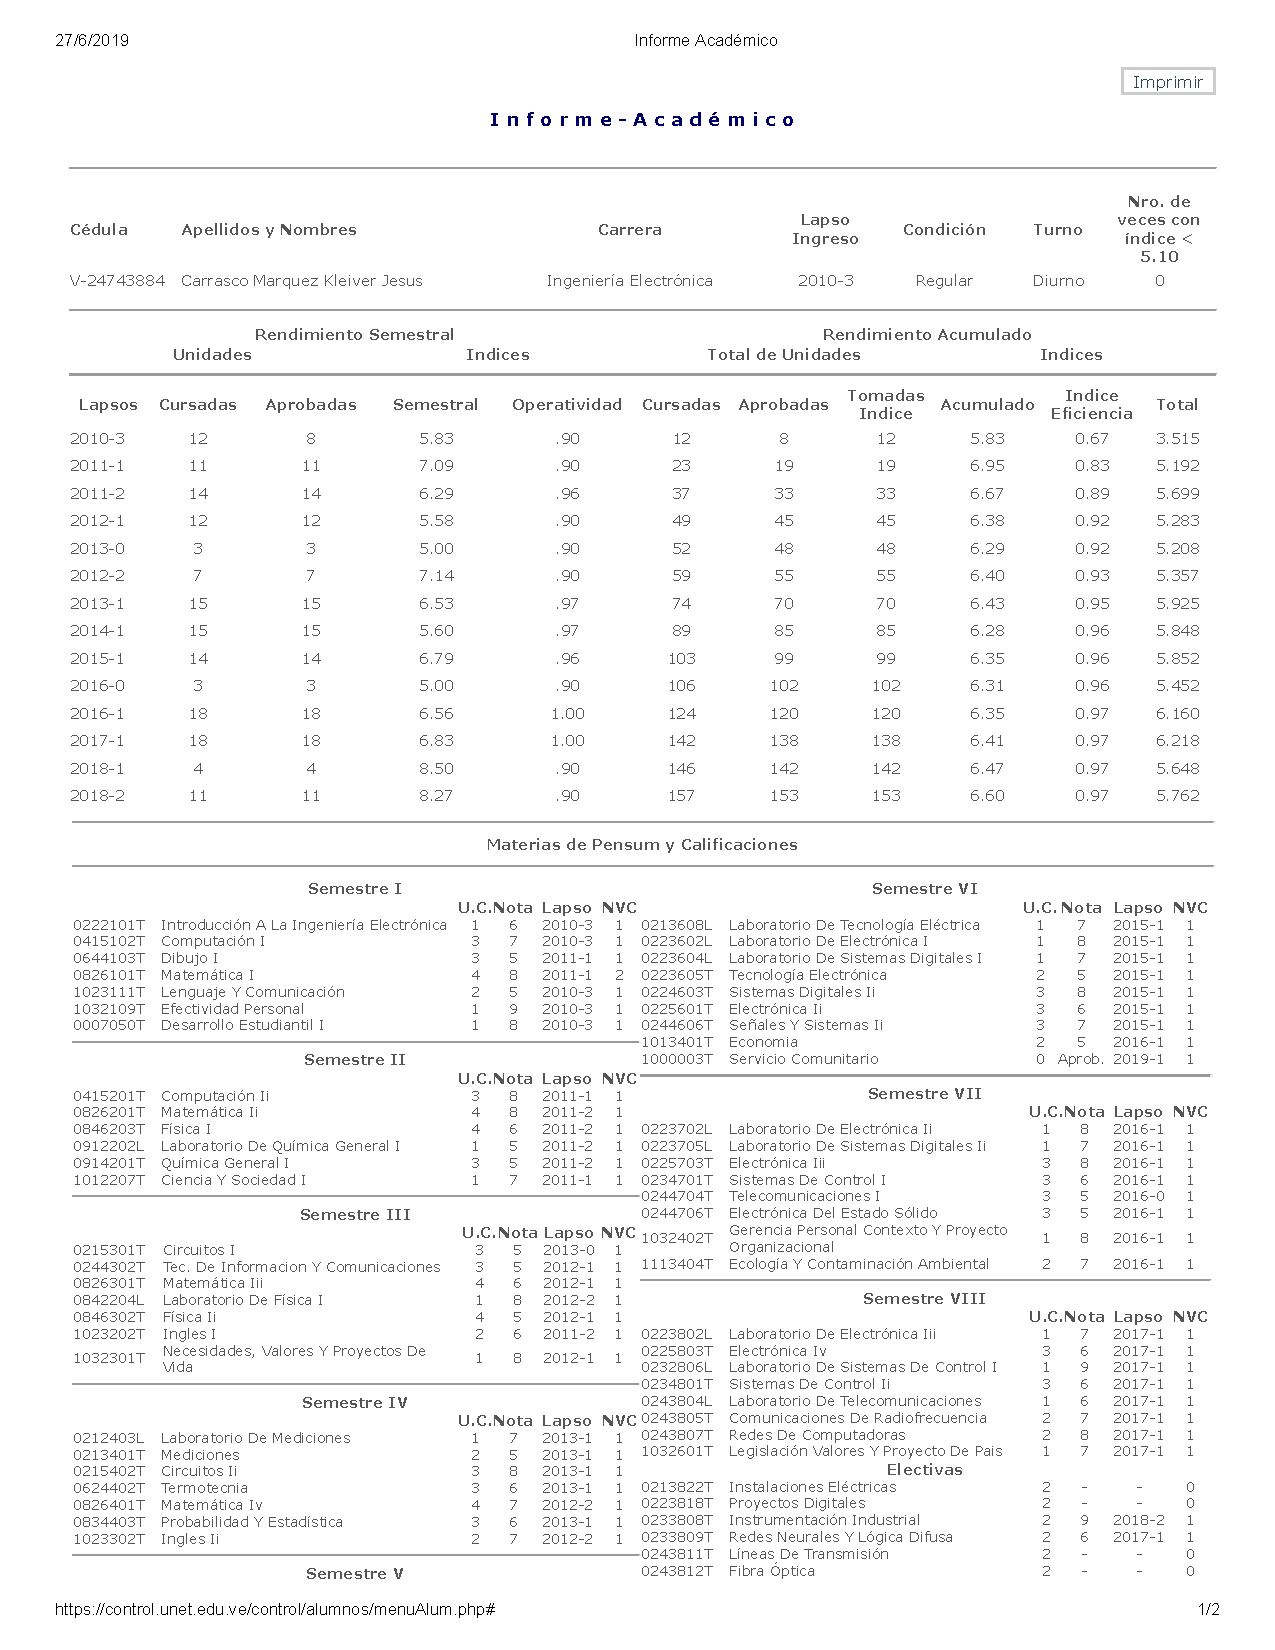
\includepdf[scale=0.7,pages=1,pagecommand={\AgregarAnexo{Informe académico}}, 
% addtotoc={1, chapter, 0,\bfseries\uppercase{Anexos}, pdf:informe}]{imagenes/informeAcademico}
% \includepdf[scale=0.7,pages=2, pagecommand={}]{imagenes/informeAcademico}
% --------------------------------------------------------------------
% Nota: Si se utiliza este código se deben comentar:
% \newpage
% \phantomsection
% \addcontentsline{toc}{chapter}{Anexos}
% --------------------------------------------------------------------

\newpage                                % Comentar si se incluye
\phantomsection                         % primero un pdf
\addcontentsline{toc}{chapter}{Anexos}  % Para evitar problemas TOC

% Para agregar anexos a la tesis
\AgregarAnexo{Codigo de los margenes de ganancia y fase}
    \begin{longlisting}
        \caption{Funcion para el calculo de los margenes de ganancia y fase}
        \label{code:1}				
        \begin{minted}[escapeinside=||,
            mathescape=true,
            autogobble=true,
            fontsize=\footnotesize,
            obeytabs=true,
            tabsize=4,
            baselinestretch=1,
			breaklines]{python}
            def margenes_ganancias(self, system, mag, phase, omega):
                """
                [Funcion para obtener el margen de ganancia y el margen de fase]
                
                :param system: [Representación del sistema]
                :type system: [LTI]
                :param mag: [Magnitud de la respuesta en frecuencia]
                :type mag: [numpyArray]
                :param phase: [Fase de la respuesta en frecuencia]
                :type phase: [numpyArray]
                :param omega: [Frecuencias utilizadas para la respuesta en frecuencia]
                :type omega: [numpyArray]
                """

                gainDb = 20 * np.log10(mag)
                degPhase = phase * 180.0 / np.pi

                # Llevando la fase a : -360 < phase < 360, para +/- 360  phase -> 0
                comp_phase = np.copy(degPhase)
                degPhase = degPhase - (degPhase/360).astype(int) * 360

                # Para evitar la deteccion de cruces al llevar las fases al rango -360 < phase < 360
                crossHack1 = np.diff(1 * (degPhase > -183) != 0)
                crossHack2 = np.diff(1 * (degPhase > -177) != 0)
                crossHack = ~crossHack1 * ~crossHack2

                # Deteccion de cruce
                indPhase = np.diff(1 * (gainDb > 0) != 0)
                indGain = np.diff(1 * (degPhase > -180) != 0)
                indGain = indGain * crossHack

                # Calculo de la respuesta en frecuencia para omega = 0 rad/s
                zero_freq_response = ctrl.evalfr(system, 0j)
                omega = np.insert(omega, 0, 0)
                zeroPhase = np.angle(zero_freq_response)
                zeroMag = np.abs(zero_freq_response)
                if zeroPhase * 180.0 / np.pi >= 180:
                    zeroPhase = zeroPhase - 2 * np.pi
                gainDb = np.insert(gainDb, 0, 20 * np.log10(zeroMag))
                degPhase = np.insert(degPhase, 0, zeroPhase * 180.0 / np.pi)

                # Verificando "cruce" por -180 grados para omega = 0 rad/s
                if zeroPhase * 180.0 / np.pi == -180:
                    indGain = np.insert(indGain, 0, True)
                else:
                    indGain = np.insert(indGain, 0, False)

                # Verificando "cruce" por 0 dB para omega = 0 rad/s
                if 20 * np.log10(zeroMag) == 0:
                    indPhase = np.insert(indPhase, 0, True)
                else:
                    indPhase = np.insert(indPhase, 0, False)

                # Margen de ganancia
                if len(omega[:-1][indGain]) > 0:
                    newGainIndex = np.argmin(np.abs(gainDb[:-1][indGain]))
                    omegaGain = omega[:-1][indGain][newGainIndex]
                    GainMargin = -gainDb[:-1][indGain][newGainIndex]
                else:
                    omegaGain = np.nan
                    GainMargin = np.infty

                # Margen de Fase
                if len(omega[:-1][indPhase]) > 0:
                    newPhaIndex = min(range(len(degPhase[:-1][indPhase])),
                                    key=lambda i: abs(np.abs(degPhase[:-1][indPhase][i]) - 180))
                    omegaPhase = omega[:-1][indPhase][newPhaIndex]
                    PhaseMargin = 180 + degPhase[:-1][indPhase][newPhaIndex]
                else:
                    omegaPhase = np.nan
                    PhaseMargin = np.infty

                return GainMargin, PhaseMargin, omegaGain, omegaPhase
        \end{minted}
    \end{longlisting}

\AgregarAnexo{Titulo de otro anexo}
    \blindtext